\documentclass{article}
\usepackage[utf8]{inputenc}
\usepackage[a4paper]{geometry}
\usepackage{graphicx}
    \graphicspath{ {Graphics/} }
\usepackage{movie15}
\usepackage{color}
\usepackage{wrapfig}
\usepackage{multirow}
\usepackage{tabu}
\usepackage[table]{xcolor}
\usepackage{subcaption}
\usepackage[colorlinks=true,urlcolor=red, pdfborder={0 0 0}]{hyperref}


\title{\huge Data Analysis and Interpretation\\
        \LARGE Report\\
        \large Week One $\vert$ Assignment One}
\author{Anish Kulkarni, Parth Jatakia, Toshi Parmar, Vedant Basu}
\date{28 September 2016}

\begin{document}
\newgeometry{left=3cm,bottom=0.1cm, right=3cm, top=3cm}
\maketitle
\newcommand\tab[1][1cm]{\hspace*{#1}}
    \begin{center} 
            \rule{16cm}{0.2pt}
    \end{center}
\section{Assigned Responsibilities}
    The following Responsibilities were designated to each team member:
    \begin{table}[h!]
    \centering
    {\rowcolors{4}{red!80!yellow!40}{red!70!yellow!30}
        \begin{tabu}to 0.8\textwidth { |X[c]||X[c]||X[c]| } 
        \hline
        Week & Role Assigned & Member\\
        \hline
        \hline
        & Leader & Vedant Basu \\ 
        & Coder & Parth Jatakia \\ 
        & Website Manager & Anish Kulkarni \\
        \multirow{-4}{10em}{\textbf Week One}& Report Writer & Toshi Parmar \\
        \hline
        \end{tabu}
        }
    \caption{Week By Week Summary of Assigned Roles}
    \label{Table:WorkAllocation}
    \end{table}
\section{Summary of Work Done}
    \begin{enumerate}
        \item \large {\textbf {Webpage Designing}}\\
            Anish designs \href{https://sites.google.com/site/ep219coursegroup/}{the webpage} considering appropriate specifications with the help of Google Sites.
        \item \large {\textbf{Familiarising with Python 2.7}}\\
            Members familiarise themselves with Python $2.7$ \& the matplotlib library by plotting Gaussian(Fig~\ref{fig:GaussianDistribution}), Binomial(Fig~\ref{fig:BinomialDistribution}) \& Poisson distributions(Fig~\ref{fig:PoissonDistribution}) for three different parameter values.
            Following are the plots for respective distributions-
            \begin{figure}[!htb]
                \fbox {\begin{minipage}{0.5\textwidth}
                    \centering
                    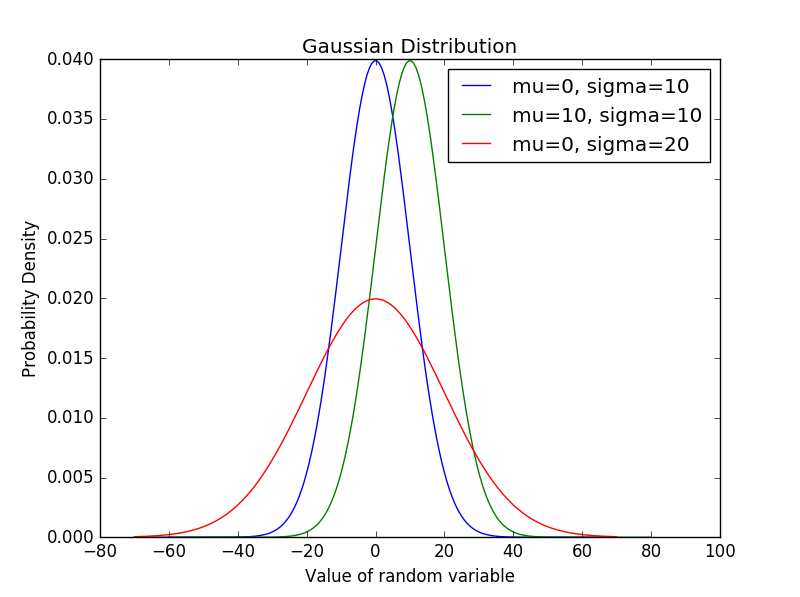
\includegraphics[width=\textwidth,height=\textheight,keepaspectratio]{gaussian}
                    \caption{Gaussian Distribution}
                    \label{fig:GaussianDistribution}
                \end{minipage}%
                }
                \fbox{\begin{minipage}{0.5\textwidth}
                    \centering
                    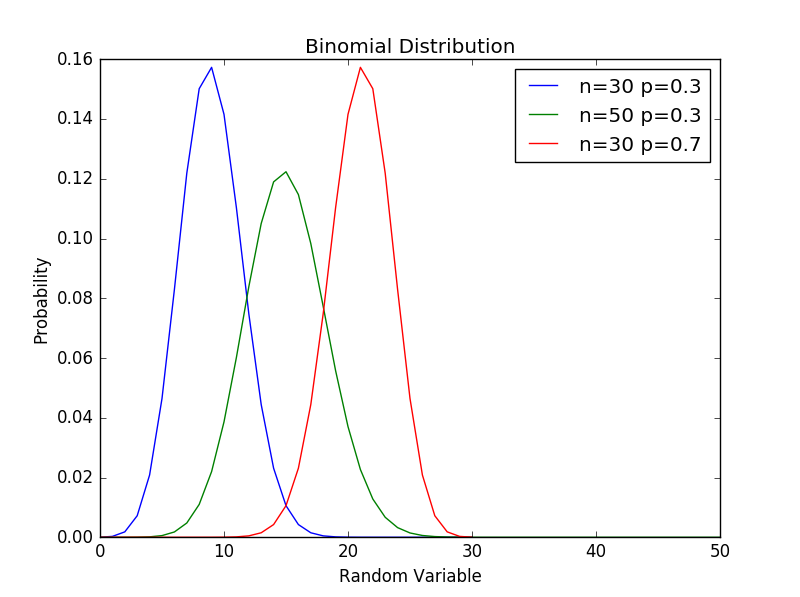
\includegraphics[width=\textwidth,height=\textheight,keepaspectratio]{binomial}
                    \caption{Binomial Distribution}
                    \label{fig:BinomialDistribution}
                \end{minipage}%
                }
            \end{figure}
            \begin{figure}[!htb]
                \fbox{\begin{subfigure}{0.31\textwidth}
                    \centering
                    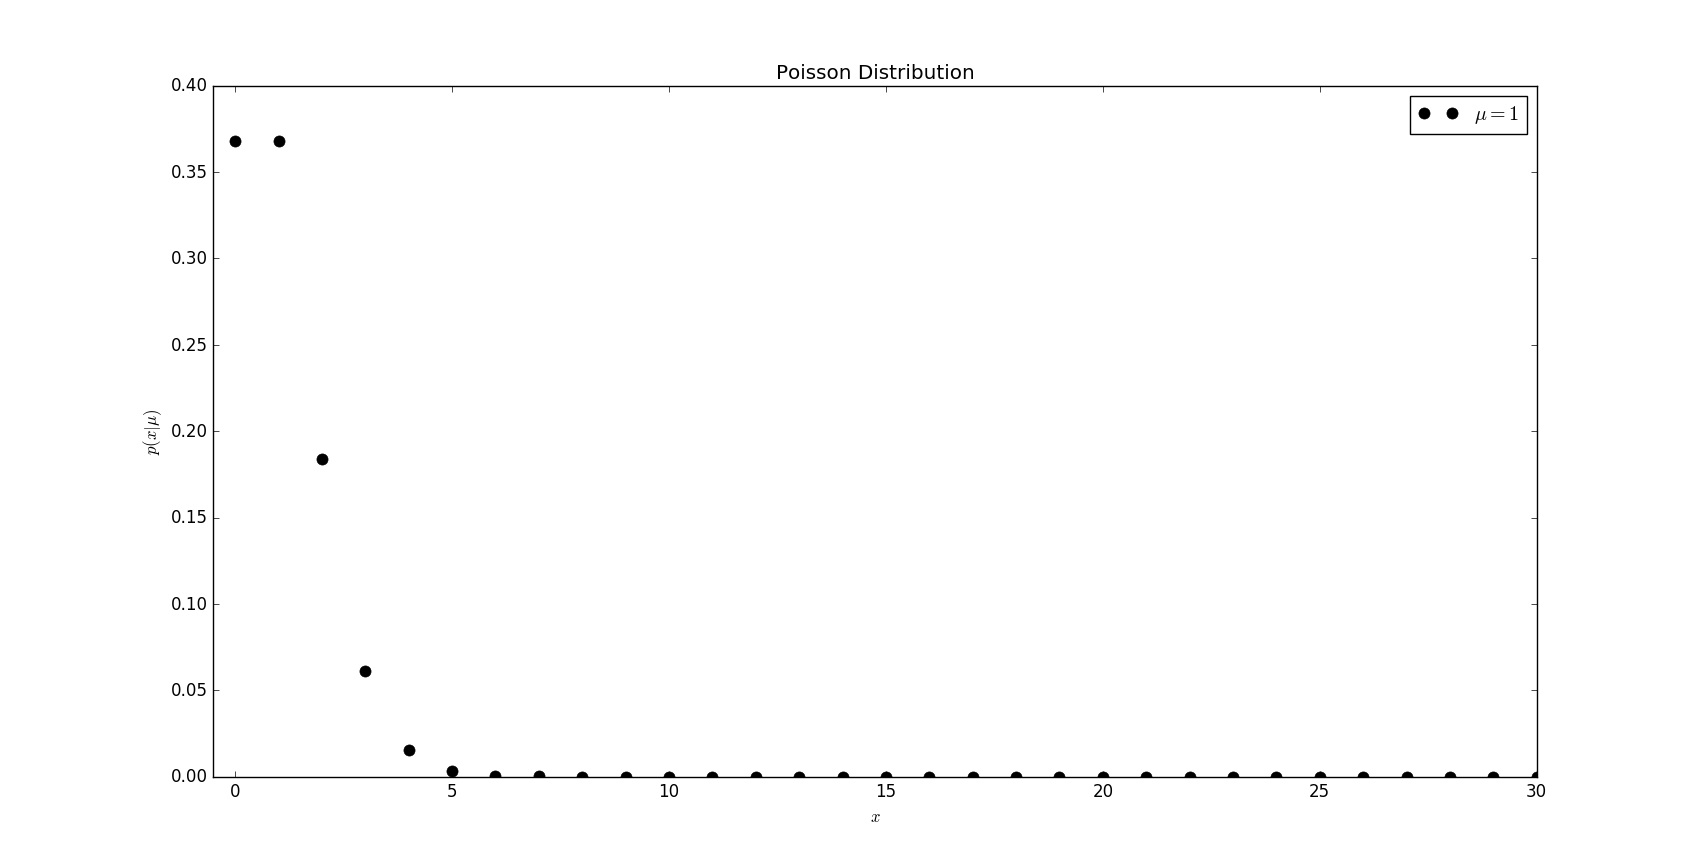
\includegraphics[width=\textwidth,height=2\textheight,keepaspectratio]{poisson_mu1}
                    \caption{Poisson Distribution, $\mu=1$}
                    \label{fig:P1Distribution}
                \end{subfigure}%
                }
                \fbox{\begin{subfigure}{0.31\textwidth}
                    \centering
                    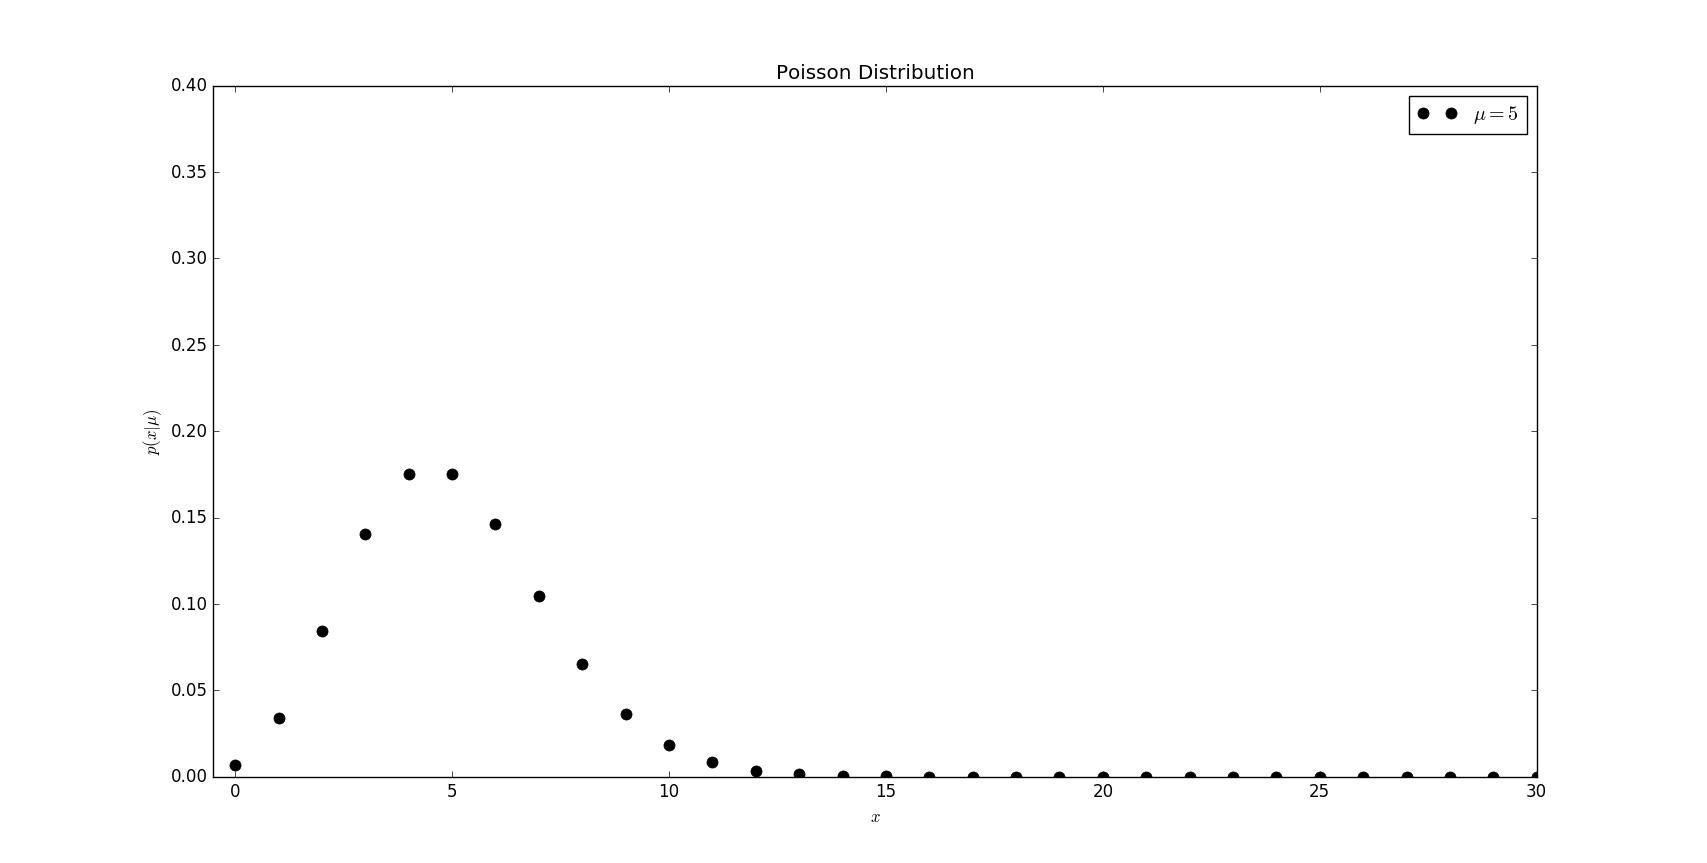
\includegraphics[width=\textwidth,height=2\textheight,keepaspectratio]{poisson_mu5}
                    \caption{Poisson Distribution, $\mu=5$}
                    \label{fig:P2Distribution}
                \end{subfigure}%
                }
                \fbox{\begin{subfigure}{0.31\textwidth}
                    \centering
                    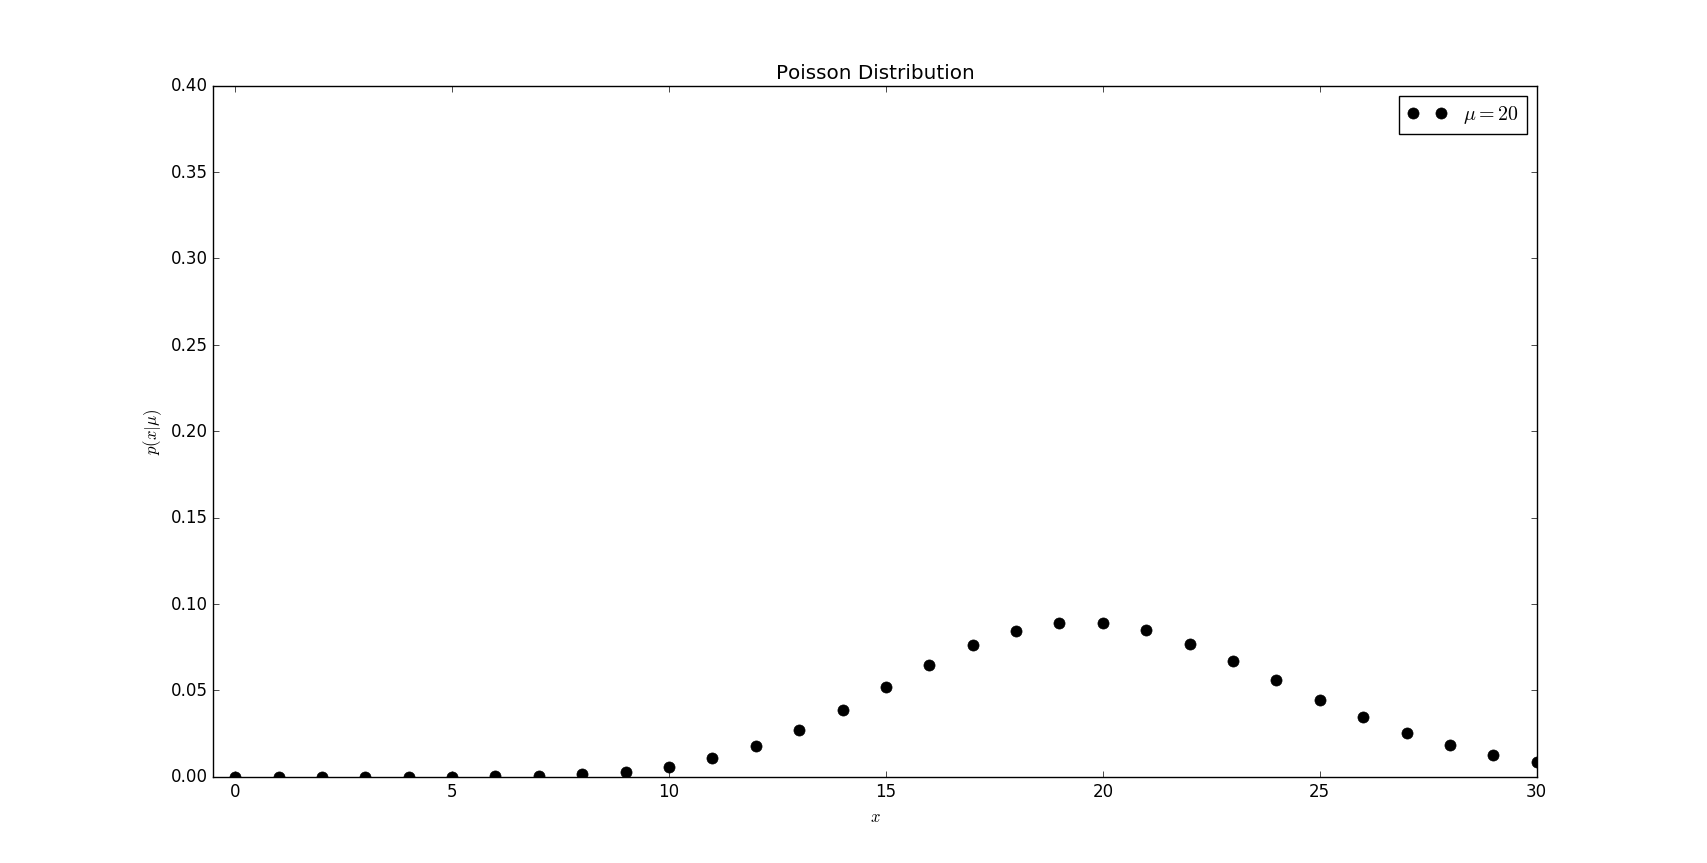
\includegraphics[width=\textwidth,height=2\textheight,keepaspectratio]{poisson_mu20}
                    \caption{Poisson Distribution, $\mu=20$}
                    \label{fig:P3Distribution}
                \end{subfigure}%
                }
            \caption{Poisson Distribution}
            \label{fig:PoissonDistribution}
            \end{figure}
        \item \large {\textbf {Algorithm for Monte-Carlo Estimation of \huge {$\pi$}}}\\
            Discussion ensued in the first meet of the team to decide an efficient algorithm to carry out the Monte-Carlo Approximation.
            Method followed is -
            \begin{enumerate}
                \item Generating random numbers.\\ Using numpy's $numpy.random.uniform(-1,1,2000)$ command which draws random numbers from a uniform distribution in the interval, 4000 random numbers for the abscissa and ordinate of points are generated.
                \item Finding $\pi$ for each iteration.\\
                No. of points which lie inside the circle (distance less than the radius of circle, $r=1$ are calculated$(n)$.
                The value of $\pi$ in this iteration is -\\
                \tab \tab \tab \fbox{ $\pi_i = 4 \frac {n}{2000.0}$}
                \item Mean value of $\pi$, Sample Width, Standard Deviation $\&$ \emph{Error}.\\
                The mean value of $\pi$ is the average of all sample values obtained from $500$ iterations of the former two steps.\\
                \tab \tab \tab \fbox{$\pi = \sum_{i=1}^{500}\pi_i $}\\
                Next up, the sample width of our distribution is estimated as the standard deviation of the $\pi$ values.\\
                And the standard deviation of our data can be estimated as-\\
                \tab \tab \tab \fbox{$ \sigma = \frac{No. of Trials}{No. of Trials - 1} $}\\
                \emph{Error} in the data is equalled to the standard deviation of our data, i.e. $\sigma$.
                \item Plotting the Histogram^{\ref{fig:PDF}}\\
                The matplotlib library's Histogram generating function is used with bin size equalled to $500^{0.5}$ (since it is an ideal central factor for $500$ observations) which approximates to 23.\\ The histogram is \emph{normalised} to $1$.\\
                \begin{figure}[!htb]
                \centering
                \includegraphics[width=0.8\textwidth,height=0.8\textheight, keepaspectratio]{PDE}
                \caption{\huge {Approximation of $\pi$}}
                \label{fig:PDF}
            \end{figure}
            \end{enumerate}
    \end{enumerate}
    
\end{document}
